%!TEX root = ClementiCooperBarba2018.tex

\subsection{Isolated nanoparticle} \label{sec:verification}

In this section we present the results of performing a verification exercise. We
compare our numerical calculations of the extinction cross-section using boundary
elements method (BEM), with analytical solutions available for spherical geometries. 

The analytical expression for the extinction cross-section of spherical geometries
provided by Mishenko \cite{Mishchenko2007} applies for all mediums. In the presence
of a lossy medium, $k^\prime$ represents the real part of the complex wave number,
otherwise $k$ is a real-valued and we take $k^\prime = k$. 


\begin{equation} 
    C_\text{ext} = \frac{4\pi a^3}{k^\prime} \operatorname{Im}\left(k^2 
                    \frac{\epsilon_p/\epsilon_m -1}{\epsilon_p/\epsilon_m -2}\right)
    \label{eq:an_sol}
\end{equation}

where $a$ is the radius of the sphere, $k$ the complex wave number ($k=k^\prime +i k^{\prime\prime}$), $\epsilon_p$ 
the dielectric constant of the particle, and $\epsilon_m$ the dielectric constant
of the host medium. 

When we applied the electrostatic approximation, the simulations reduces to a 
sphere under a constant electric field, like presented in Fig. \ref{fig:np_elec_field}.

\begin{figure}[h] %  figure placement: here, top, bottom, or page
   \centering
   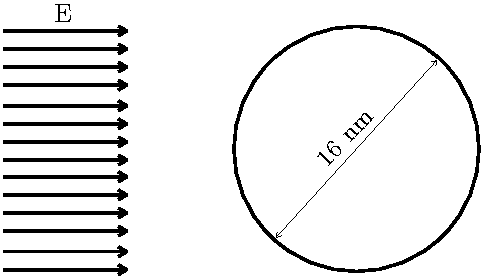
\includegraphics[width=0.3\textwidth]{sphere_field_8nm.pdf} 
   \caption{Spherical nanoparticle in a constant electric field.}
   \label{fig:np_elec_field}
\end{figure}

Figure \ref{fig:error_sphere_Ag} shows a grid convergence study of the extinction
cross-section of a silver spherical nanoparticle of radius $8 \, nm$ immersed in water
under a z-polarized electric field with a wavelength of $380 nm$ and intensity of 
$-0.0037 e/({\AA}^2 \, \epsilon_0)$. Under these conditions water has a dielectric
constant of $1.7972 \, + \, 8.5048^{-09}i$ \cite{JohnsonChristy1972} and silver of
$-3.3877 \, + \, 0.1922i$ \cite{HaleQuerry1972}. In these simulations we used $K=4$ 
Gauss quadrature points per far-away elements, $K_{fine} = 37$ Gauss quadrature points
per elements for near singular integrals, $Nk = 9$ Gauss quadrature points per 
triangle edge for semi-analytical integration in the singular elements, $P=15$ for 
the order of expansion in treecode, and a GMRES tolerance of $10^{-5}$. We
performed the simulation for meshes of 512, 2048, 8192 and 32768 elements. The 
error calculation uses the analytical solution $C_{ext} = 1854.4765 \; nm^2$ 
obtained using equation \eqref{eq:an_sol}.

\begin{figure}[h] %  figure placement: here, top, bottom, or page
   \centering
   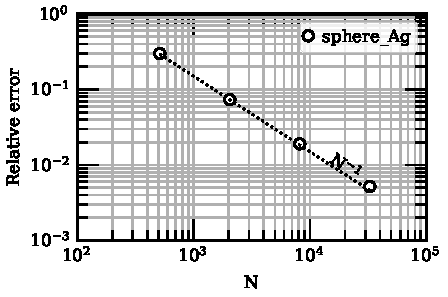
\includegraphics[width=0.45\textwidth]{convergence_sph_Ag_R8_w=380.pdf} 
   \caption{Grid-convergence study of extinction cross-section of a spherical silver
            nanoparticle.}
   \label{fig:error_sphere_Ag}
\end{figure}

The computed order of convergence is $0.98$ and the $1/N$ slope in Fig. \ref{fig:error_sphere_Ag}
show that the numerical solutions computed with \pygbe for isolated spheres are
correctly resolved by the meshes.

The percentage errors for the different meshes are presented in Table. \ref{table:err_iso_sphere}.

\begin{table}[h]
    \centering
    \caption{\label{table:err_iso_sphere} Percentage error of isolated silver sphere.} 
    \begin{tabular}{c c}
    \hline%\toprule
    N & \% error \\
    \hline%\midrule
     $512$ & $29.86$ \\
     $2048$ & $7.33$ \\
     $8192$ & $1.9$ \\
     $32768$ & $0.52$ \\
    \hline%\bottomrule
    \end{tabular}
\end{table}


To complete the process of verification we perform simulations of the extinction 
cross-section of the isolated sphere for a spectrum of wavelengths. To ensure 
errors $<2\%$ we use the mesh of $N=32768$ elements. 

Figure \ref{fig:verif_sphere} shows the extinction cross-section of the isolated
sphere of Fig.\ref{fig:np_elec_field} as a function of wavelength. The values of 
the dielectric constants for each wavelength were obtained by interpolation of 
experimental data \cite{JohnsonChristy1972, HaleQuerry1972}.


\begin{figure}[h] %  figure placement: here, top, bottom, or page
   \centering
   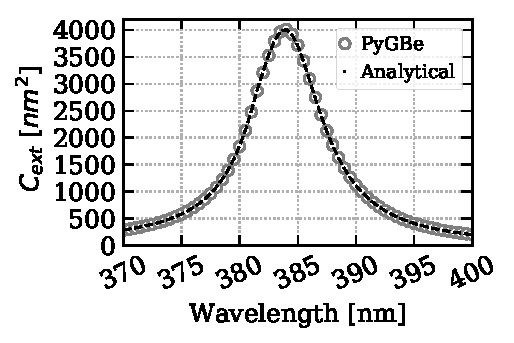
\includegraphics[width=0.45\textwidth]{silver_NP_verification.pdf} 
   \caption{Extinction cross-section as a function of wavelength for a $8 \, nm$
            silver sphere immersed in water}
   \label{fig:verif_sphere}
\end{figure}

We can see good agreement between simulations and analytical results, proving
that we are achieving an accurate numerical solution of the mathematical model. The 
peak in the extinction cross-section indicates that the plasmons of the metallic
nanoparticle are resonating with the incoming electric field.


\subsection{LSPR response to BSA} \label{sec:lspr_response}

Localized Surface Plasmon Resonance biosensors detect a target molecule by monitoring
plasmon resoncance frequency changes due to the proximity of the target to the metallic
nanoparticle. In this section we perform simulations that show how our BEM approach
can be used to model the response of LSPR biosensors.

To ensure that we are achieving an accurate numerical solution, we performed a 
convergence analysis of the system showed in Figure \ref{fig:setup_conv}. Where
we use as analyte a Bovine Serum Albumina (PDB code 4FS5) protein. The BSA mesh
was generated using the open source software Nanoshaper (missing how to cite - not
reported in their webpage). Nanoshaper takes as input the coordinates and radius
of the atoms in the crystal structure, whcih were extracted from the the van der
Waals radii and charges of the atoms file (\texttt{pqr}) generated using 
\texttt{pdb2pqr} \cite{Dolinsky04}, with the built-in \texttt{amber} force field.

Since we compute the extinction cross section over the sphere nanoparticle, we 
set a fixed mesh density for the protein and varied the refinement over the
sphere (meshes of 512, 2048, 8192 and 32768 elements). After studying different 
cases we decide to use a mesh of density two triangles per ${\AA}^2$ for 
the protein, resulting in a mesh of $N_{prot} = 98116$. 


\begin{figure}[h] %  figure placement: here, top, bottom, or page
   \centering
   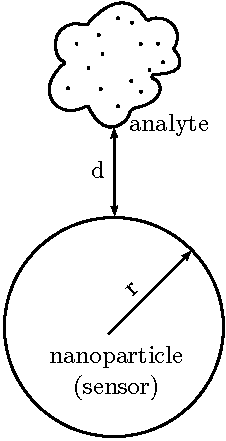
\includegraphics[width=0.15\textwidth]{protein_sphere_sketch.pdf} 
   \caption{Setup for convergence analysis of the response calculation.}
   \label{fig:setup_conv}
\end{figure}

We repeated the conditions and parameters for the simulations used in the isolated
sphere presented in Section \ref{sec:verification}. In this case we added the 
dielectric constant for the protein $2.7514 + 0.2860i$ extracted from the 
functional relationship provided by Pahn, et al. \cite{PahnETal2013}, and the 
distance between the sensor and the analyte is $d=1 \, nm$. The error calculation
uses the Richardson extrapolation value of the extinction cross-section as a
reference, $C_{ext}= 1778.7259 \, nm^2$


\begin{figure}[h] %  figure placement: here, top, bottom, or page
   \centering
   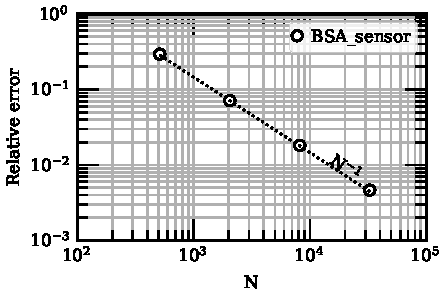
\includegraphics[width=0.45\textwidth]{convergence_bsa_sensor_R8_d=1_w=380.pdf} 
   \caption{Grid-convergence study of extinction cross-section of a spherical silver
            nanoparticle with a BSA protein at $d=1 \, nm$.}
   \label{fig:error_sphere-bsa}
\end{figure}

The computed order of convergence in this case is $0.99$, and we can see in 
Figure \ref{fig:error_sphere-bsa} that the error decays with the number
of boundary elements ($1/N$), which is consistent with our verification 
results of Section \ref{sec:verification}. This proves that the
numerical solutions computed with \pygbe are correctly resolved by the meshes.

The percentage errors for the different meshes are presented in Table. \ref{table:err_bsa_sensor}.

\begin{table}[h]
    \centering
    \caption{\label{table:err_bsa_sensor} Percentage error of BSA-sensor sytem Fig. \ref{setup_conv}.} 
    \begin{tabular}{c c}
    \hline%\toprule
    N & \% error \\
    \hline%\midrule
     $512$ & $29.39$ \\
     $2048$ & $7.13$ \\
     $8192$ & $1.82$ \\
     $32768$ & $0.46$ \\
    \hline%\bottomrule
    \end{tabular}
\end{table}

Before the study of the LSPR response to the to the BSA protein, we performed a 
relaxation of parameters to optimize run time without compromising our small
percentage error. We reduced the density of the protein mesh to one element per
${\AA}^2$ ($N_{prot}=45140$) and fixed the sphere mesh to $N_{sensor}=32768$. We
set $K=4$ Gauss quadrature points per far-away elements, $K_{fine} = 19$ Gauss
quadrature points per elements for near singular integrals, $Nk = 9$ Gauss 
quadrature points per triangle edge for semi-analytical integration in the 
singular elements, $P=6$ for the order of expansion in treecode, and a GMRES 
tolerance of $10^{-3}$. These choices result in a percentage error of $\sim\%0.6$
and the time of each computation is approximately $7.5 min$ in a \texttt{NVIDIA Tesla K40 GPU}
card. 



\begin{figure*}[h] %  figure placement: here, top, bottom, or page
   \centering
   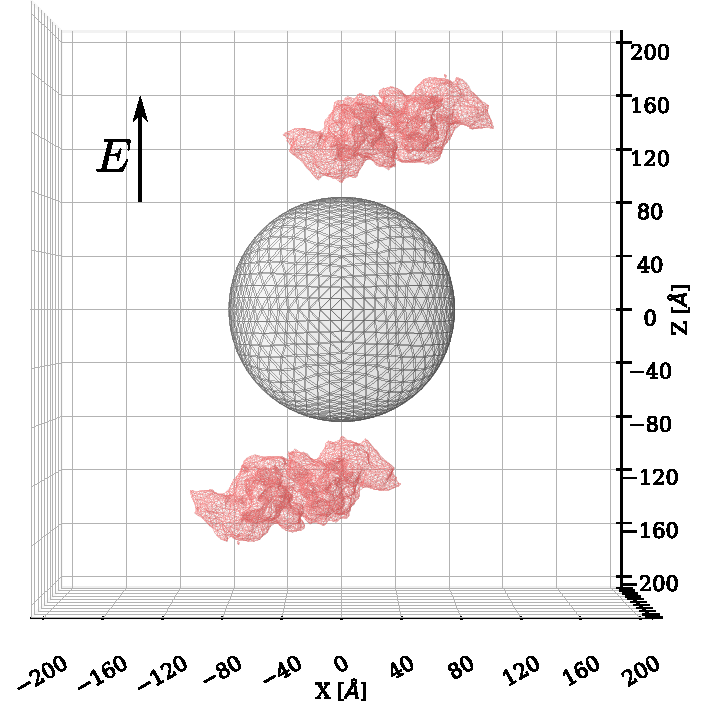
\includegraphics[width=0.5\textwidth]{2prot_1nm_z_R8nm.pdf} 
   \caption{Sensor protein display: BSA located at 1 nm of the nanoparticle in the
            z-direction}
   \label{fig:display_z}
\end{figure*}



\begin{figure}[h] %  figure placement: here, top, bottom, or page
   \centering
   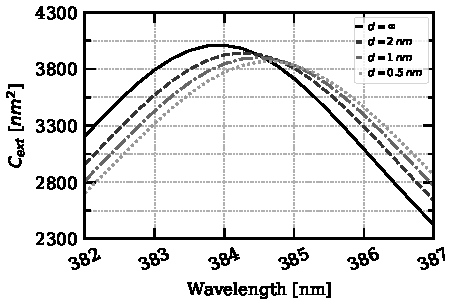
\includegraphics[width=0.45\textwidth]{2pz_lspr_response.pdf} 
   \caption{}
   \label{fig:dist_response}
\end{figure}



\begin{figure}[h] %  figure placement: here, top, bottom, or page
   \centering
    %since we have dots in the names we need to enclose what is before the 
    %extension in { }
   \includegraphics[width=0.45\textwidth]{{2pz_00_ef-0.0037_R8nm}.pdf} 
   \caption{}
   \label{fig:2pz_response}
\end{figure}



\begin{figure*}[h]

   \centering
   \subfloat{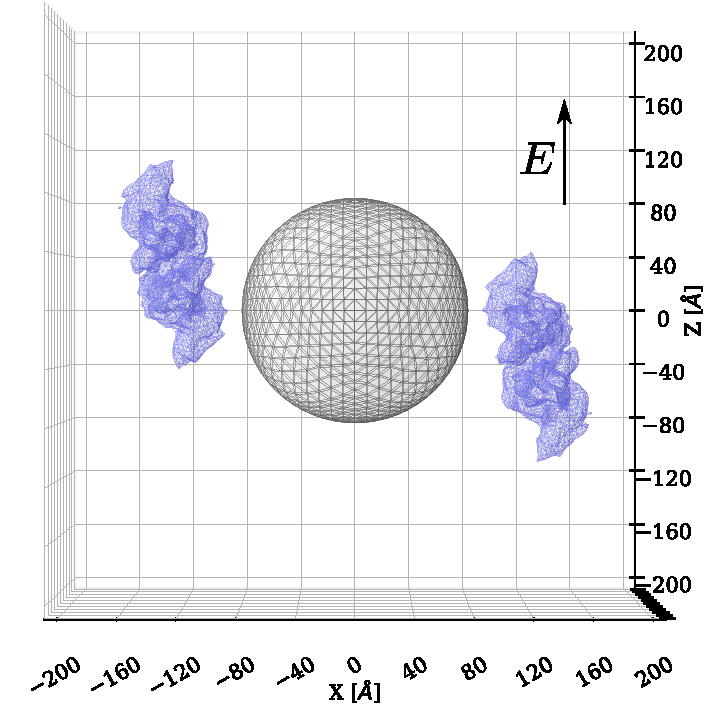
\includegraphics[width=0.49\textwidth]{2prot_1nm_x_R8nm.pdf}} 
%   \caption{Sensor protein display: BSA located at 1 nm of the nanoparticle in the
%            x-direction}
   %\label{fig:display_x}
    \quad
   \subfloat{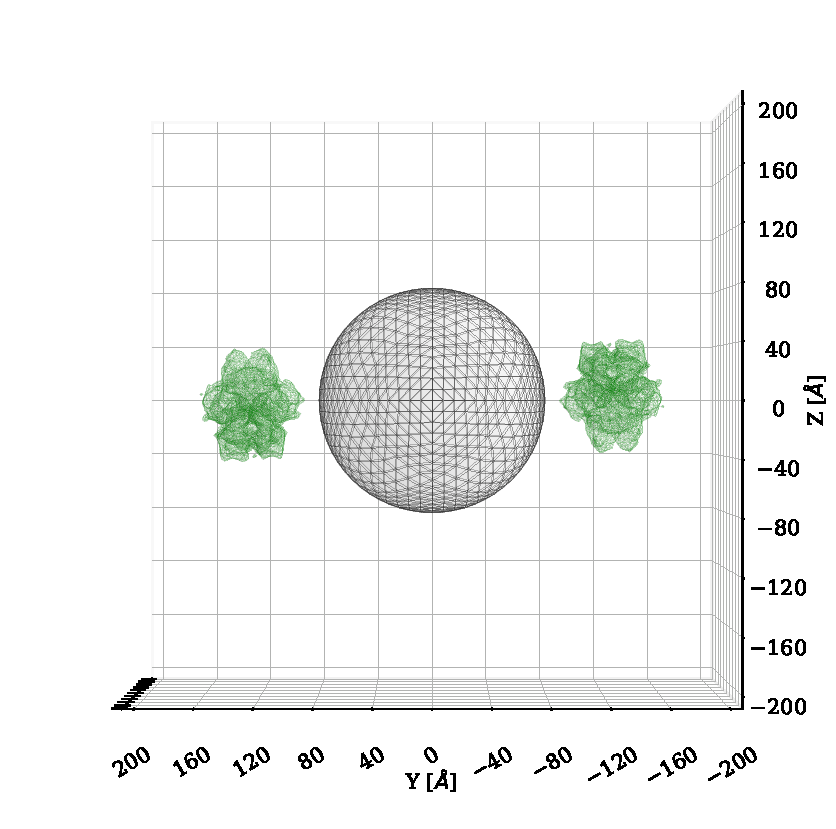
\includegraphics[width=0.49\textwidth]{2prot_1nm_y_R8nm.pdf}} 
%   \caption{Sensor protein display: BSA located at 1 nm of the nanoparticle in the
%            y-direction}
   \label{fig:display_y}
    \caption{Sensor protein display: BSA located at 1 nm of the nanoparticle in the
            x-direction (left) and y-direction (right)}

\end{figure*}


the variation of the extinction cross-section with respect to the wavelength, for each of the distances shown above. The red shift in the resonance frequency and the decrement of the peak in the presence of the analyte agrees with the behavior observed in experiments perform by Tang et al. \cite{TangETal2010}. This indicates that our boundary element method approach, using electrostatic approximation, is capable of reproducing characteristic resonance frequency shift in LSPR biosensors.




Experiments suggests that the distance between the nanoparticle and the analyte affects the sensitivity of the sensor \cite{HaesETal2004}, and these proof-of-concept calculations show that our approach can be use to study sensitivity versus distance, using electrostatics.




Generate distance variation plot. 


Fig result of 2px and 2py

\begin{figure}[h] %  figure placement: here, top, bottom, or page
   \centering
   \includegraphics[width=0.45\textwidth]{{2px_00_ef-0.0037_R8nm}.pdf} 
   \caption{}
   \label{fig:2px_response}
\end{figure}

\begin{figure}[h] %  figure placement: here, top, bottom, or page
   \centering
   \includegraphics[width=0.45\textwidth]{{2py_00_ef-0.0037_R8nm}.pdf} 
   \caption{}
   \label{fig:2py_response}
\end{figure}



